\documentclass{standalone}


\usepackage{tikz}
\usetikzlibrary{calc, shapes, arrows, decorations.pathmorphing}


\begin{document}

	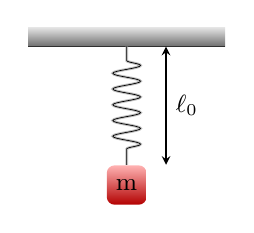
\begin{tikzpicture}
	
	\node[] (tetocenter) at (0,0) {};
	
	
	\coordinate (centroN) at (0,0) {};
	\coordinate (massaN) at (0,-1.5) {};
	\coordinate (tetoL) at (-1.25,0) {};
	\coordinate (tetoR) at (1.25,0) {};
	
	\draw[-] (tetoL)--(tetoR) ;
	
	\node[rectangle, bottom color=gray!50!black, top color=gray!30, opacity=0.75, minimum width=2.5cm, minimum height=2, anchor=south] (teto) at (0,0) {};
	\draw[-,line width=1.pt, color=gray!50, decorate,decoration={snake,amplitude=5pt,pre length=5pt,post length=5pt, segment length=2mm}] (centroN) -- (massaN); 
	\draw[-,line width=0.25pt, color=black, decorate,decoration={snake,amplitude=5pt,pre length=5pt,post length=5pt, segment length=2mm}] (centroN) -- (massaN); 
	
	\node[rectangle, rounded corners=1mm, minimum width=0.5cm, 
	minimum height=0.5cm, top color=red!30, bottom color=red!70!black, anchor=north] (massa) at (massaN.south) [font=\small]{m};
	

	\draw[stealth-stealth] ($(massaN)+(0.5,0)$)-- node [right, font=\small] {$\ell_0$}($(centroN)+(0.5,0)$);
	
	\end{tikzpicture}



\end{document}
